
% ------------ Notes on the proposed new array representation
% \begin{itemize}
% \item An @Array@ is a partial function from a rectangular range of indices to values.  
% \item Unlike Repa 2, the bottom LH corners of the range is not necessarily zero; instead @extent@ returns an @Range@ (figure 1) which gives the two corners.
% \item A partitioned @(P r1 r2)@ is just a pair of arrays described by @r1@, @r2@. 
% \item Each of the sub-arrays is self-describing; it is rectangular, has an extent (usually smaller than its parent!), etc
% \item Note how beautifully simple @fillP@ becomes in Figure 7!
% \end{itemize}
% ------------- End of new array rep


Figure~\ref{figure:UglySpecialisation} shows the ugly array specialisation code we used to use to implement map. The hope was that @map@ would be specialised to the number of regions in the input array, but if @mR@ and @mapGen@ are inlined before this specialisation this causes explosion in the intermediate core code.


% --------------------------------------------------------
\begin{figure}
\begin{small}
\begin{code}
data Array sh a
  = Array        { arrayExtent   :: sh
                 , arrayRegions  :: [Region sh a] }
data Region sh a
  = Region       { regionRange   :: Range sh
                 , regionGen     :: Generator sh a }
data Range sh
  = RangeAll
  | RangeRects   { rangeMatch    :: sh -> Bool
                 , rangeRects    :: [Rect sh] }

data Rect sh   = Rect sh sh

data Generator sh a
  = GenManifest  { genVector :: Vector a }

  | forall cursor.
    GenCursored  { genMake   :: sh -> cursor
                 , genShift  :: sh -> cursor -> cursor
                 , genLoad   :: cursor -> a }
\end{code}
\end{small}
\caption{Recursive array types}
\end{figure}

% --------------------------------------------------------
\begin{figure}
\begin{small}
\begin{code}
map :: (Shape sh, Elt a, Elt b) => (a -> b)
    -> Array sh a -> Array sh b

map f (Array sh regions)
 = Array sh (mapRegions regions)
 where	
  mapRegions rs
   = case rs of
      []               -> []
      [r]              -> [mR r]
      [r1, r2]         -> [mR r1, mR r2]
      [r1, r2, r3]     -> [mR r1, mR r2, mR r3]
      [r1, r2, r3, r4] -> [mR r1, mR r2, mR r3, mR r4]
      _                -> mapRegions' rs

  mapRegions' []      = []
  mapRegions' (r:rs') = mR r : mapRegions' rs'

  mR  = mapRegion
  mapRegion (Region range gen)
      = Region range (mapGen gen)

  mapGen gen
   = case gen of
      GenManifest vec -> ...
      GenCursor makeCursor shiftCursor loadElem -> ...
\end{code}
\end{small}
\caption{Ugly array specialisation}
\label{figure:UglySpecialisation}
\end{figure}


% -----------------------------------------------------------------------------
In some cases the GHC simplifier will unfold the definition to eliminate these tests, but this can lead to explosion in the size of the intermediate program, which we discuss in \REF \simon{What is REF?  Do we want to distract attention here?}. As mentioned in \REF, we can step around this problem in client code by manually specialising the function to only accept the array representation we plan on passing to it:
%
\begin{small}
\begin{code}
    doubleZip1 arr1@Manifest{} arr2@Manifest{}
     = force $ map (* 2) $ zipWith (+) arr1 arr2
\end{code}
\end{small}
% 
\simon{Obvious problem: crashes if given a @Delayed@ array!  We must point this out.}
Now the test happens once per array rather than once per array \emph{element}.
This is was a serviceable approach for Repa 1, but adding the support for partitioned arrays in Repa 2 increased the complexity of the array representation and the size of the required patterns along with it.  The array representation used in Repa 2 is shown in Figure \ref{figure:Repa2}. In this case the array is partitioned into several regions, where each can be independently manifest, or represented using a \emph{cursor function}. Cursored arrays are a generalisation of delayed arrays which are used to optimise the compilation of programs using stencil convolution. The @genMake@ field converts an index to a cursor value which points to a particular element of the array. The @genShift@ function offsets the cursor to point to a different element, and @genLoad@ retrieves the pointed-to element. As described in \cite{Lippmeier:Stencil}, given an existing element function  @elemFn :: sh -> e@ we can wrap this as a cursored array by using the generator @(GenCursored id addDim elemFn)@, where @addDim :: sh -> sh -> sh@ adds two indices component-wise.

Adapting the @doubleZip@ function above to the Repa 2 array representation yields:
%
\begin{small}
\begin{code}
    doubleZip2 arr1@(Array _ [Region _ GenManifest{}]) 
               arr2@(Array _ [Region _ GenManifest{}])
     = force $ map (* 2) $ zipWith (+) arr1 arr2
\end{code}
\end{small}
%
With the Repa 2 array representation, the addition of array partitioning means that the @Manifest@ constructor that we need to match against is buried within a larger structure. Although adding the required pattern matches to @doubleZip1@ (using Repa 1) was not overly cumbersome, the corresponding patterns in @doubleZip2@ (using Repa 2) are more of a syntactic burden than we would reasonably expect users to put up with. \simon{And it still crashes on unexpected arguments!}


% -----------------------------------------------------------------------------
\begin{figure}
\begin{small}
\begin{code}
data Array sh a
   = Array       { arrayExtent  :: sh
                 , arrayRegions :: [Region sh a] }
data Region sh a
   = Region      { regionRange  :: Range sh
                 , regionGen    :: Generator sh a }
data Range sh 
   = RangeAll
   | RangeRects  { rangeMatch   :: sh -> Bool
                 , rangeRects   :: [Rect sh] }
data Rect sh
   = Rect sh sh

data Generator sh a
   = GenManifest { genVector   :: Vector a }    
   | forall cursor. 
     GenCursored { genMake     :: sh -> cursor
                 , genShift    :: sh -> cursor -> cursor
                 , genLoad     :: cursor -> a }
\end{code}
\end{small}
\caption{Repa 2 array representation}
\label{figure:Repa2}
\end{figure}


% -----------------------------------------------------------------------------
In addition to the cumbersome pattern matches described in the previous section, using the array representation of Figure \ref{figure:Repa2} makes it difficult to write code that is generic in the number of array regions. The problem is that Repa style array fusion depends critically on inlining, but recursive functions that operate on the list of regions in the @arrayRegions@ field of @Array@ will not be completely unfolded by the GHC simplifier. This is because GHC is a general purpose compiler, and is rightly concerned about compile-time divergence, as well as the size of the resulting binary.

The utility of partitioned arrays is that they allow each region to be defined via a separate client-provided function. In our work on stencil convolution, \cite{Lippmeier:Stencil} the result of applying a stencil to a source array is one consisting of two regions: the \emph{inner region}, where the applied stencil is guaranteed to fall entirely within the source array; and the \emph{border region} where some elements of the stencil may fall outside. The border regions itself is defined by four separate rectangles (@Rect@s from Figure \ref{figure:Repa2}), corresponding to the edges of a 2-dimensional array. Each region is defined via a separate element function, wrapped up as a @Generator@, with the one for the inner region able to be more fully optimised as it does not need to worry about handling the border conditions.

The fact that each region is defined by a separate element function implies that a separate instance of @force@ must be unfolded for each one. Unfortunately, due to the restrictions on inlining mentioned previously, we could not write a recursive function over the list of regions, or the @Rect@ defining each region, and instead manually unfolded our array filling functions a fixed number of times:
%
\begin{small}
\begin{code}
  fillRegion2P :: (Int -> a -> IO ()) 
               -> DIM2 -> Region DIM2 a -> IO ()
  fillRegion2P write sh@(DIM2 h w) (Region range gen)
   = case range of
      RangeAll -> ...
      RangeRects _ [r1]
       -> do fillRect2 write sh gen r1
      RangeRects _ [r1, r2]
       -> do fillRect2 write sh gen r1
             fillRect2 write sh gen r2
      RangeRects _ [r1, r2, r3]
       -> do fillRect2 write sh gen r1
             fillRect2 write sh gen r2
             fillRect2 write sh gen r3
      ...
\end{code}
\end{small}
%
Here, @fillRegion2P@ takes a parameter function used to write an element into the destination array, the size of the overall array, and the definition of an array region as a list of @Rect@s. It then calls @fillRect2@ which uses the region's element generator to fill the area of the array defined by each @Rect@.

Besides being not being generic in the number of @Rect@s, heavy use of inlining tends to cause an explosion in the size of the intermediate code for programs written in this way. During compilation, the array that @fillRegion2P@ is eventually applied to will contain a fixed number of @Rect@s. Many copies of @fillRect2@, along with the associated element function will be unfolded and optimised during compilation, only to be discarded when the simplifier finally specialises each instance @fillRegion2P@ for the number of @Rect@s it is applied to. This problem can be partly managed using by staging the order in which each function is inlined, using the inliner phase numbers described in \CITE. However, in our experience this is difficult to get right, mainly due to the fact that the GHC simplifier performs inlining interspersed with other transformations. This makes it hard to reason about what exactly happened during compilation, even given a dump of the intermediate representation of the program after each phase. In \REF we show how to use type indices to ensure that each array filling function is unfolded only the correct number of times.


% -----------------------------------------------------------------------------
Continuing the cons-list analogy, if the @P@ representation tag corresponds to a type-level @Cons@ constructor, then @X@ corresponds to @Nil@. The @X@ type is the representation tag for arrays whose elements are completely undefined. Indexing into an undefined array invokes Haskell's @error@ function. An example partitioned array is as follows:
\par
\begin{small}
\begin{code}
 arr1 :: Array (P D (P D X)) DIM2 Int
 arr1 = let size   = DIM2 10 10
           range1 = ...; fn1 = ...
           range2 = ...; fn2 = ...
       in  APart size range1 (fromFunction size fn1)
         $ APart size range2 (fromFunction size fn2)
         $ AUndefined size
\end{code}
\end{small}
\par
Here we have defined an array consisting of two delayed partitioned, terminated by an undefined partition. Note that the @apartSize@ field contains the size of the entire array, and not just the particular particular partition it is attached to. We do this so our array filling functions can determine the total size of the array given just the outermost partition. It is a run-time error if the @apartSize@ fields in a partitioned array do not match. Alternatively, we could eliminate the @apartSize@ field and have our filling functions compute the overall size of the array from the embedded range fields. We stick to the former option for simplicity. 

Instead of using an undefined array to terminate the partitioning, it is also reasonable to use a final delayed array. For example:
%
\begin{small}
\begin{code}
 arr2 :: Array (P D D) DIM2 Int
 arr2 = let size   = DIM2 10 10
            range1 = ...; fn1 = ...
            range2 = ...; fn2 = ...
        in APart size range1 (fromFunction size fn1)
         $ fromFunction size fn2
\end{code}
\end{small}
%
In practice we prefer to use the former version with the undefined array, because it makes debugging errors in the range definitions easier. If the range definitions are smaller than they should be, meaning the overall array definition has ``gaps'' between the partitions, then indexing undefined elements falls-through to the undefined array and we get an explicit error message. In contrast, if we were to terminate the partitioning with a delayed array, then if there are bugs in the range code then it will be indexed at unexpected positions, who's element values may not be well-defined.


% -----------------------------------------------------------------------------
With the partitioned array of \S\ref{section:Partitioned} we are able to compute the internal and border regions of an array with functions specialised to each region. However, with just the definitions given previously, the partitioning can be ``hidden'' when we perform further operations to a partitioned array. Consider the following example which performs a single iteration in a program to solve the Laplace equation in a 2-dimensional grid. This benchmark was discussed in our earlier work of \cite{Lippmeier:Stencil}.
%
\par 
\begin{small}
\begin{code}
 type Image = Array U DIM2 Float
 
 relaxLaplace :: Image -> Image -> Image -> Image
 relaxLaplace arrBoundValue arrBoundMask arr
  = computeP  $ zipWith (+) arrBoundValue
              $ zipWith (*) arrBoundMask
              $ map (/ 4)
              $ mapStencil2 (BoundConst 0)
                [stencil2| 0 1 0
                           1 0 1 
                           0 1 0 |] arr
\end{code}
\end{small}
\par
%
\simon{Here we use @computeP@ which we have not introduced.  We have only talked of @computeIOP@.}
As specified in Figure~\ref{figure:Cursored}, the @mapStencil@ function takes a description of how to handle boundary conditions, a stencil definition, and a source array. In the above example the stencil is defined with syntactic sugar provided via Template Haskell \cite{Lippmeier:Stencil}. The subsequent @map@ re-normalises the result of the stencil application, so that if the source array elements lie in the range @[0..1]@ then so will the result elements. The two applications of @zipWith@ apply internal boundary conditions. The @boundMask@ array contains @0@ values where the boundary conditions apply, and @1@ otherwise. The @arrBoundValue@ array contains the value of the boundary where it applies, and @0@ otherwise.

Although the result of @mapStencil2@ has type @Array PD5 DIM2 a@, with @PD5@ as per Figure~\ref{figure:Cursored}, the result of applying @map@ and @zipWith@ has type @Array D DIM2 a@. As we can see from Figure~\ref{figure:BulkOperations}, the definitions of @map@ and @zipWith@ are such that the result array is necessarily delayed. This means that the final call to @computeP@ cannot ``see'' the partitioning or cursoring of the array produced by @mapStencil2@, and thus the computation method defaults to the standard one for delayed arrays. The result array will be divided evenly between the threads and each block computed sequentially, instead of using cursored evaluation for the inner partition, and other specialised functions for the borders. In this example, the fact that computation defaults to this method will be \emph{slower} than if @mapStencil2@ had not used partitioning originally. This is because evaluation must now use the @rangeMatch@ predicate from Figure~\ref{figure:Partitioned} to associate each element with the partition that defines it, so that the correct element function can be determined.

To solve this problem, we need to ensure that application of @map@, @zipWith@ preserve the partitioning and cursoring of the array representation. We do this via the @Combine@ class given in Figure~\ref{figure:Combine} which provides a mapping between the source and result representations of the bulk operations @map@ and @zipWith@. With @Combine r1 a b@, the parameter @r1@ gives the index of the source array, while @a@ and @b@ are the element types of the source and result arrays respectively. The representation of the result is given via an associated type synonym \cite{Chakravarty:AssocTypeSynonyms} 
named @TR@ (short for Target Representation). 

As per Figure~\ref{figure:Combine}, the @Combine@ instances for manifest arrays can just call the original @map@ and @zipWith@ functions. The important instances are the ones for Cursored (@C@) and Partitioned (@P@) arrays. In the instance for Cursored arrays we perform a @cmap@ by composing the worker function with the one from the array representation that loads the value at the given cursor position (@loadc@). This ensures that the array still maps cursor positions to element values. 

The instance for Partitioned @(P)@ arrays recursively applies the worker function to each partition. Note that in the type synonym instance for partitioned arrays, the @P@ constructor is at top-level on the right of the definition @P (TR r1) (TR r2)@. This makes @cmap@ a \emph{homomorphism} (a structure preserving map).

Note that the Partitioned instance of @czipWith@ is right-biased, meaning that only the structure of the second source array is preserved. Preserving the partitioning of \emph{both} source arrays would be more complicated. For example:
%
\begin{center}
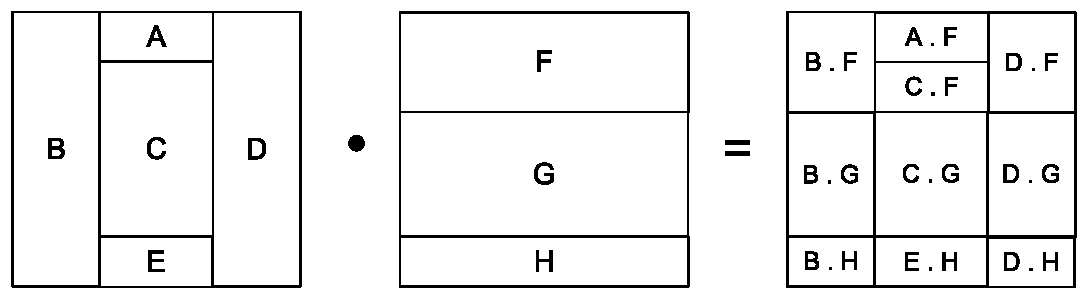
\includegraphics[scale=0.3]{figs/guiding-zipwith-partitions.pdf}
\end{center}
%
The number of extant partitions in the result array depends on the size and shape of the partitions in both source arrays. To produce the correct number of loops during code-fusion we would need to know the shape of each partition at compile-time. Note that while the shape of each partition is a value, the number of partitions is a type, which makes this a dependently-typed problem. 

In Repa 2 the @zipWith@ function was also right-biased, but in a monomorphic way that did not appear in the type (or the documentation, sorry!) of this function. As with @fillRegion2P@ from \S\ref{section:Explosion}, we hand-specialised it to a fixed number of cases which was again non-general, and prone to code-explosion.

% \begin{small}
% \begin{code}
% zipWith :: (a -> b -> c) 
%         -> Array sh a -> Array sh b -> Array sh c
% zipWith f (Array sh2 [_]) 
%  (Array sh1 [ Region g21 (GenCursor mk21 _ ld21)
%             , Region g22 (GenCursor mk22 _ ld22)]) = ...
% zipWith f arr1 arr2 = ...
% \end{code}
% \end{small}

Similarly to \S\ref{section:Partitioned}, the instances from Figure~\ref{figure:Combine} will now be unfolded the correct number of times, guided by the representation tags in the array type. The fact that @czipWith@ is right-biased is also visible from its type signature. Finally, note that Repa 3 includes the original @zipWith@ as well as our new @czipWith@ function. With plain @zipWith@ if the overall shape of the source arrays is different then the shape of the result is their intersection. Performing this intersection is possible when there is no internal partitioning to worry about. In contrast, @czipWith@  preserves the partitioning of the second source array, but the overall shape of both source arrays must match. 
